% science_template.tex
% See accompanying readme.txt for copyright statement, change log etc.

% Any modification of this template, including writing a paper using it,
% MUST rename the file i.e. use a different file name.

%%%%%%%%%%%%%%%% START OF PREAMBLE %%%%%%%%%%%%%%%

% Basic setup. Authors shouldn't need to adjust these commands.
% It's annoying, but please do NOT strip these into a separate file.
% They need to be included in this .tex for our production software to work.

% Use the basic LaTeX article class, 12pt text
\documentclass[12pt]{article}

% Science uses Times font. If you don't have this installed (most LaTeX installations will be
% fine) or prefer the old Computer Modern fonts, comment out the following line
\usepackage{newtxtext,newtxmath}
% Depending on your LaTeX fonts installation, you might get better results with one or both of these:
%\usepackage{mathptmx}
%\usepackage{txfonts}

% Allow external graphics files
\usepackage{graphicx}

%%% Tompkins IMPORTS
% Mathematics and Times-style fonts
\usepackage{amsmath}

% Use US letter sized paper with 1 inch margins
\usepackage[letterpaper,margin=1in]{geometry}

%%% Tompkins imports
\usepackage{tikz}
\usepackage{newfloat}
\usetikzlibrary{decorations.pathreplacing}

\setlength{\oddsidemargin}{0in}
\setlength{\evensidemargin}{0in}
\setlength{\textwidth}{6.5in}
\setlength{\topmargin}{-0.5in}
\setlength{\textheight}{9in}
\setlength{\parindent}{0pt}
\setlength{\parskip}{0.9em}
\setlength{\emergencystretch}{3em}

\newcommand{\photoplaceholder}[1]{%
    \begin{center}
    \fbox{\begin{minipage}[c][2.2in][c]{0.78\textwidth}
    \centering\textbf{PHOTO PLACEHOLDER}\\[8pt]#1
    \end{minipage}}
    \end{center}}

% Drawings receive their own “Example” counter.
\DeclareFloatingEnvironment[
    name=Example,
    listname={List of Examples}
]{example}

% Double line spacing, including in captions
\linespread{1.5} % For some reason double spacing is 1.5, not 2.0!

% One space after each sentence
\frenchspacing

% Abstract formatting and spacing - no heading
\renewenvironment{abstract}
{\quotation}
{\endquotation}

% No date in the title section
\date{}

% Reference section heading
\renewcommand\refname{References and Notes}

% Figure and Table labels in bold
\makeatletter
\renewcommand{\fnum@figure}{\textbf{Figure \thefigure}}
\renewcommand{\fnum@table}{\textbf{Table \thetable}}
\makeatother



% Provides the \url command, and fixes a crash if URLs or DOIs contain underscores
\usepackage{url}

%%%%%%%%%%%% CUSTOM COMMANDS AND PACKAGES %%%%%%%%%%%%

% Authors can define simple custom commands e.g. as shortcuts to save on typing
% Use \newcommand (not \def) to avoid overwriting existing commands.
% Keep them as simple as possible and note the warning in the text below.

% Example:
\newcommand{\pcc}{\,cm$^{-3}$}	% per cm-cubed

% If your BibTeX uses shortcuts for journal names, define them here e.g.
% \newcommand{\apj}{Astrophys.~J.}

% Please DO NOT import additional external packages or .sty files.
% Those are unlikely to work with our conversion software and will cause problems later.
% Don't add any more \usepackage{} commands.


%%%%%%%%%%%%%%%% TITLE AND AUTHORS %%%%%%%%%%%%%%%%

% Title of the paper.
% Keep it short and understandable by any reader of Science.
% Avoid acronyms or jargon. Use sentence case.
\def\scititle{
    \textbf{ON THE BASIS OF MATHEMATICS}
}
% Store the title in a variable for reuse in the supplement (otherwise \maketitle deletes it)
\title{\bfseries \boldmath \scititle}

% Author and institution list.
% Institution numbers etc. should be hard-coded, do *not* use the \footnote command.
\author{
% You can write out first names or use initials - either way is acceptable, but be consistent
    Christopher Robinson Tompkins III, Independent, Richmond, VA\and\
% Do not include street addresses, postal codes etc.
%
% Identify at least one corresponding author, with contact email address
    Corresponding author. Email: chtompki@apache.org,\\ chtompki@vt.edu, tompkinscr@vcu.edu
% Joint contributions can be indicated like this
}

%%%%%%%%%%%%%%%%% END OF PREAMBLE %%%%%%%%%%%%%%%%


%%%%%%%%%%%%%%%% START OF MAIN TEXT %%%%%%%%%%%%%%%
\begin{document}

% Insert the title and author list
    \maketitle

% Abstract, in bold
% There are strict length limits, and not all formats have abstracts.
% Consult the journal instructions to authors for details.
% Do not cite any references in the abstract.
    \begin{abstract} \bfseries \boldmath
        We explore and explain the fundamentals of mathematical language(s). Simply.
    \end{abstract}


    \textbf{(0)}
    \begin{center}
        \emph{Dedicated to the memory of those killed at Virginia Tech,\\
        and in solidarity with those who were injured, their families,\\
        and the Virginia Tech community.}
        \qquad\\
        \emph{I would like to acknowledge the following people that helped me along the way: mom, dad, Margo, Nora,
            Griff Elder (and the 2007 VT Mathematics department and all my friends from there), George McNulty (and the 2009 USC Mathematics department and all my friends from there),
            Andy Lewis (and the VCU 2026 Mathematics Department and all my friends from there), and those at NASA whom I've worked with.}
        \qquad\\
        \emph{Note. The examples and the idea about using photos for self reference as opposed to using the drawn
        hand came from ChatGPT. THE IDEAS!!!}
    \end{center}

    \textbf{(1)}
    \section*{MATHS}

    We have a considerable number of open problems with regards to mathematics.
    Though there is one above the rest that confuses us. It is simple, it's been
    used and referred to numerous times.

    \[
        P:\neg P
        \qquad\text{or}\qquad
        \text{``THIS SENTENCE IS FALSE\ldots''}
    \]

    Yes considerable work has been done to ``RECTIFY'' or FIX this seemingly
    fundamental flaw in logic. But, in 1934 through his numbering system and
    Turing's machine, Kurt G\"odel showed this sentence to be TRUE.

    Now we have a slightly different opinion of the matter, it is the beginning of
    the language (NATURAL or MECHANICAL) and its collection of ideas. We ask is $P$
    TRUE or FALSE, but that's not the answer at all -- because it is both TRUE AND
    FALSE simultaneously and this is good because it gives us the concepts of

    \[
        \underline{\text{TRUE}},\quad
        \underline{\text{FALSE}},\quad
        \underline{\text{AND}},\quad
        \underline{\text{OR}},\quad
        \underline{\text{NOT}}
    \]

    implicitly. Yet we're missing something, even though we have TRUTH defined,
    what is it? A SYSTEM OF REFERENTIAL CAPACITY, so let's define one.

    \newpage

    So we begin with the idea of two bounded continuums

    \begin{center}
        \begin{tikzpicture}[x=0.9cm,y=0.9cm]
            \draw[thick] (0,0) rectangle (8,4);
            \fill[black!78] (0,0) rectangle (4,4);
            \draw[thick] (4,0) -- (4,4);
            \node[align=center] at (-1.55,2) {DARK\\CONTINUUM};
            \node[align=center] at (9.55,2) {LIGHT\\CONTINUUM};
            \foreach \y in {-0.75,-1.35,-1.95} {
                \fill (2,\y) circle (0.16);
                \draw[thick] (6,\y) circle (0.16);
            }
        \end{tikzpicture}
    \end{center}
    OR perhaps
    \begin{center}
        
\begin{tikzpicture}
            \def\radius{2}

            % Outer black circle
            \fill[black] (0,0) circle[radius=\radius];

            % White half and the two interlocking curves
            \fill[white]
            (0,\radius)
            arc[start angle=90, end angle=270, radius=\radius]
            arc[start angle=270, end angle=90, radius=\radius/2]
            arc[start angle=-90, end angle=90, radius=\radius/2]
            -- cycle;

            % Opposite-colored dots
            \fill[black] (0, 1) circle[radius=0.25];
            \fill[white] (0,-1) circle[radius=0.25];

            % Outer border
            \draw[black, line width=1pt] (0,0) circle[radius=\radius];
        \end{tikzpicture}
    \end{center}

    WE CHOOSE DARK AND LIGHT TO DIFFERENTIATE OUR CONTINUUMS OUT OF NATURAL
    CONVENIENCE. WE THEN ALLOW ``DOTS'' OR ``ATOMS'' (IF WE WANT TO GET TO
    RUSSELL \& TARSKI) TO BE PULLED OR CREATED FROM EITHER OF THE CONTINUUM.
    AN ATOM OR DOT WE TAKE TO BE A CONTIGUOUS PIECE OF CONTINUUM, JUST RELATIVELY
    SMALLER.

    Some quick examples of the power for referential capacity follow as,

    \textbf{(2)}
% S drwaing
    \begin{example}[htbp]
        \centering
        \begin{tikzpicture}
            \def\cellsize{1}
            \def\dotradius{0.25} % Half the cell's effective radius

            % All-white 5×5 chessboard
            \fill[white] (0,0) rectangle (5,5);
            \draw[black, line width=0.8pt]
            (0,0) grid[step=\cellsize] (5,5);

            % Dots covering the top, middle, and bottom rows
            \foreach \y in {0.5,2.5,4.5}{
                \foreach \x in {0.5,1.5,2.5,3.5,4.5}{
                    \fill[black] (\x,\y) circle[radius=\dotradius];
                }
            }

            % Leftmost cell of the second row
            \fill[black] (0.5,3.5) circle[radius=\dotradius];

            % Rightmost cell of the fourth row
            \fill[black] (4.5,1.5) circle[radius=\dotradius];
        \end{tikzpicture}
        \caption{Description of the drawing.}
        \label{ex:drawing-label}
    \end{example}

% DOTTED TABLE DRAWING:
    \begin{example}[htbp]
        \centering
        \resizebox{\textwidth}{!}{%
            \begin{tikzpicture}[
                dot/.style={
                    circle,
                    fill=black,
                    inner sep=0pt,
                    minimum size=3.2pt
                },
                x=5.2mm,
                y=5.2mm
            ]

        \newcommand{\dotsat}[1]{%
            \foreach \x/\y in {#1}
            \node[dot] at (\x,\y) {};
        }

        % T
        \begin{scope}[shift={(0,0)}]
            \dotsat{
                0/4,1/4,2/4,3/4,4/4,
                2/3,2/2,2/1,2/0
            }
        \end{scope}

        % A
        \begin{scope}[shift={(6,0)}]
            \dotsat{
                0/0,0/1,0/2,
                1/3,2/4,3/3,
                4/2,4/1,4/0,
                1/2,2/2,3/2
            }
        \end{scope}

        % B
        \begin{scope}[shift={(12,0)}]
            \dotsat{
                0/0,0/1,0/2,0/3,0/4,
                1/4,2/4,3/4,4/3,
                1/2,2/2,3/2,
                4/1,1/0,2/0,3/0
            }
        \end{scope}

        % L
        \begin{scope}[shift={(18,0)}]
            \dotsat{
                0/4,0/3,0/2,0/1,0/0,
                1/0,2/0,3/0,4/0
            }
        \end{scope}

        % E
        \begin{scope}[shift={(24,0)}]
            \dotsat{
                0/4,1/4,2/4,3/4,4/4,
                0/3,
                0/2,1/2,2/2,3/2,
                0/1,
                0/0,1/0,2/0,3/0,4/0
            }
        \end{scope}

        % Dotted arrow
        \begin{scope}[shift={(31,0)}]
            \dotsat{
                0/3,1/3,2/3,3/3,
                0/1,1/1,2/1,3/1,
                4/4,5/3,6/2,5/1,4/0
            }
        \end{scope}

        % Dotted table
        \begin{scope}[shift={(42,0)}]

            % Hollow, right-leaning tabletop
            \foreach \r in {0,...,3}{
                \foreach \c in {0,...,6}{
                    \ifnum\r=0
                    \node[dot]
                    at ({\c+0.45*\r},{4+\r}) {};
                    \else\ifnum\r=3
                    \node[dot]
                    at ({\c+0.45*\r},{4+\r}) {};
                    \else
                             \ifnum\c=0
                             \node[dot]
                             at ({\c+0.45*\r},{4+\r}) {};
                             \else\ifnum\c=6
                             \node[dot]
                             at ({\c+0.45*\r},{4+\r}) {};
                             \fi\fi
                    \fi\fi
                }
            }

            % Table legs
            \dotsat{
                0/3,0/2,0/1,0/0,
                6/3,6/2,6/1,6/0,
                1.35/3,1.35/2,1.35/1,
                7.35/6,7.35/5,7.35/4,7.35/3
            }
        \end{scope}

            \end{tikzpicture}%
        }
        \caption{Dots forming the word ``TABLE,'' followed by an arrow
        and a representation of a table.}
        \label{ex:dotted-table}
    \end{example}

    \begin{figure}[htbp]
        \centering
        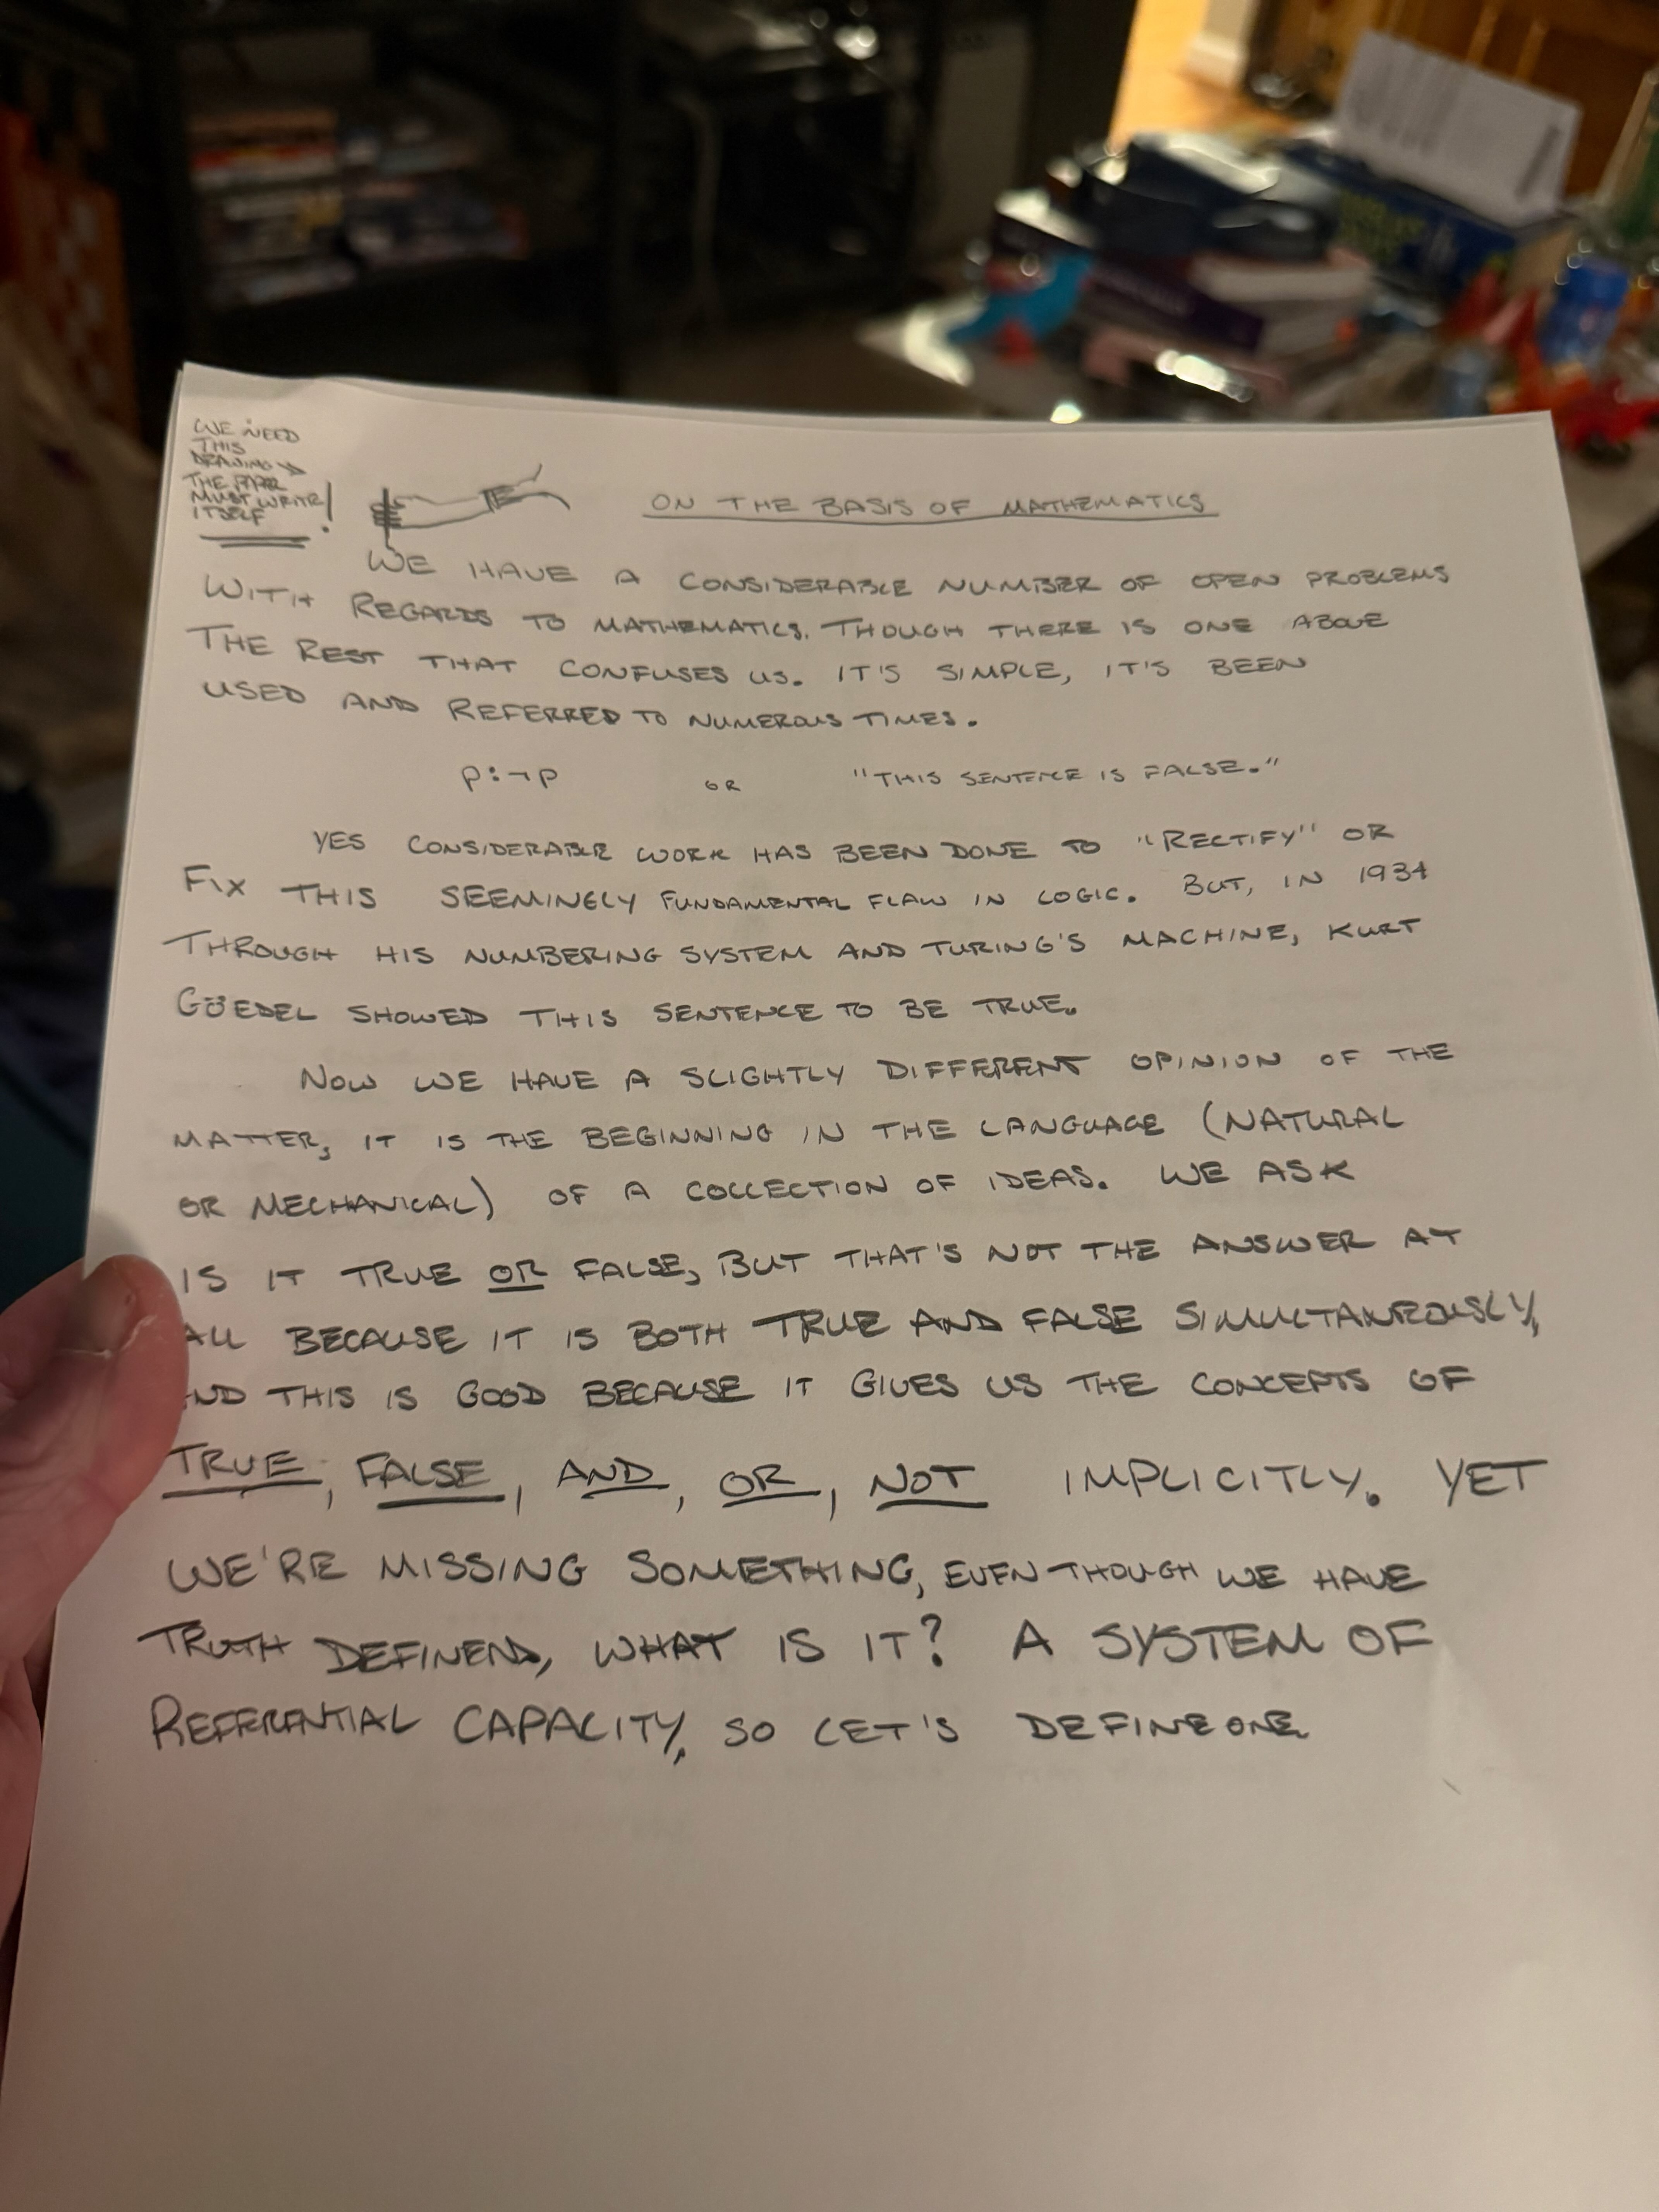
\includegraphics[width=0.4\textwidth]{math1_small.jpeg}
        \caption{Figure 1: A photo of page 1 of this handwritten paper for the purposes of self referentiality}
    \end{figure}

    \begin{figure}[htbp]
        \centering
        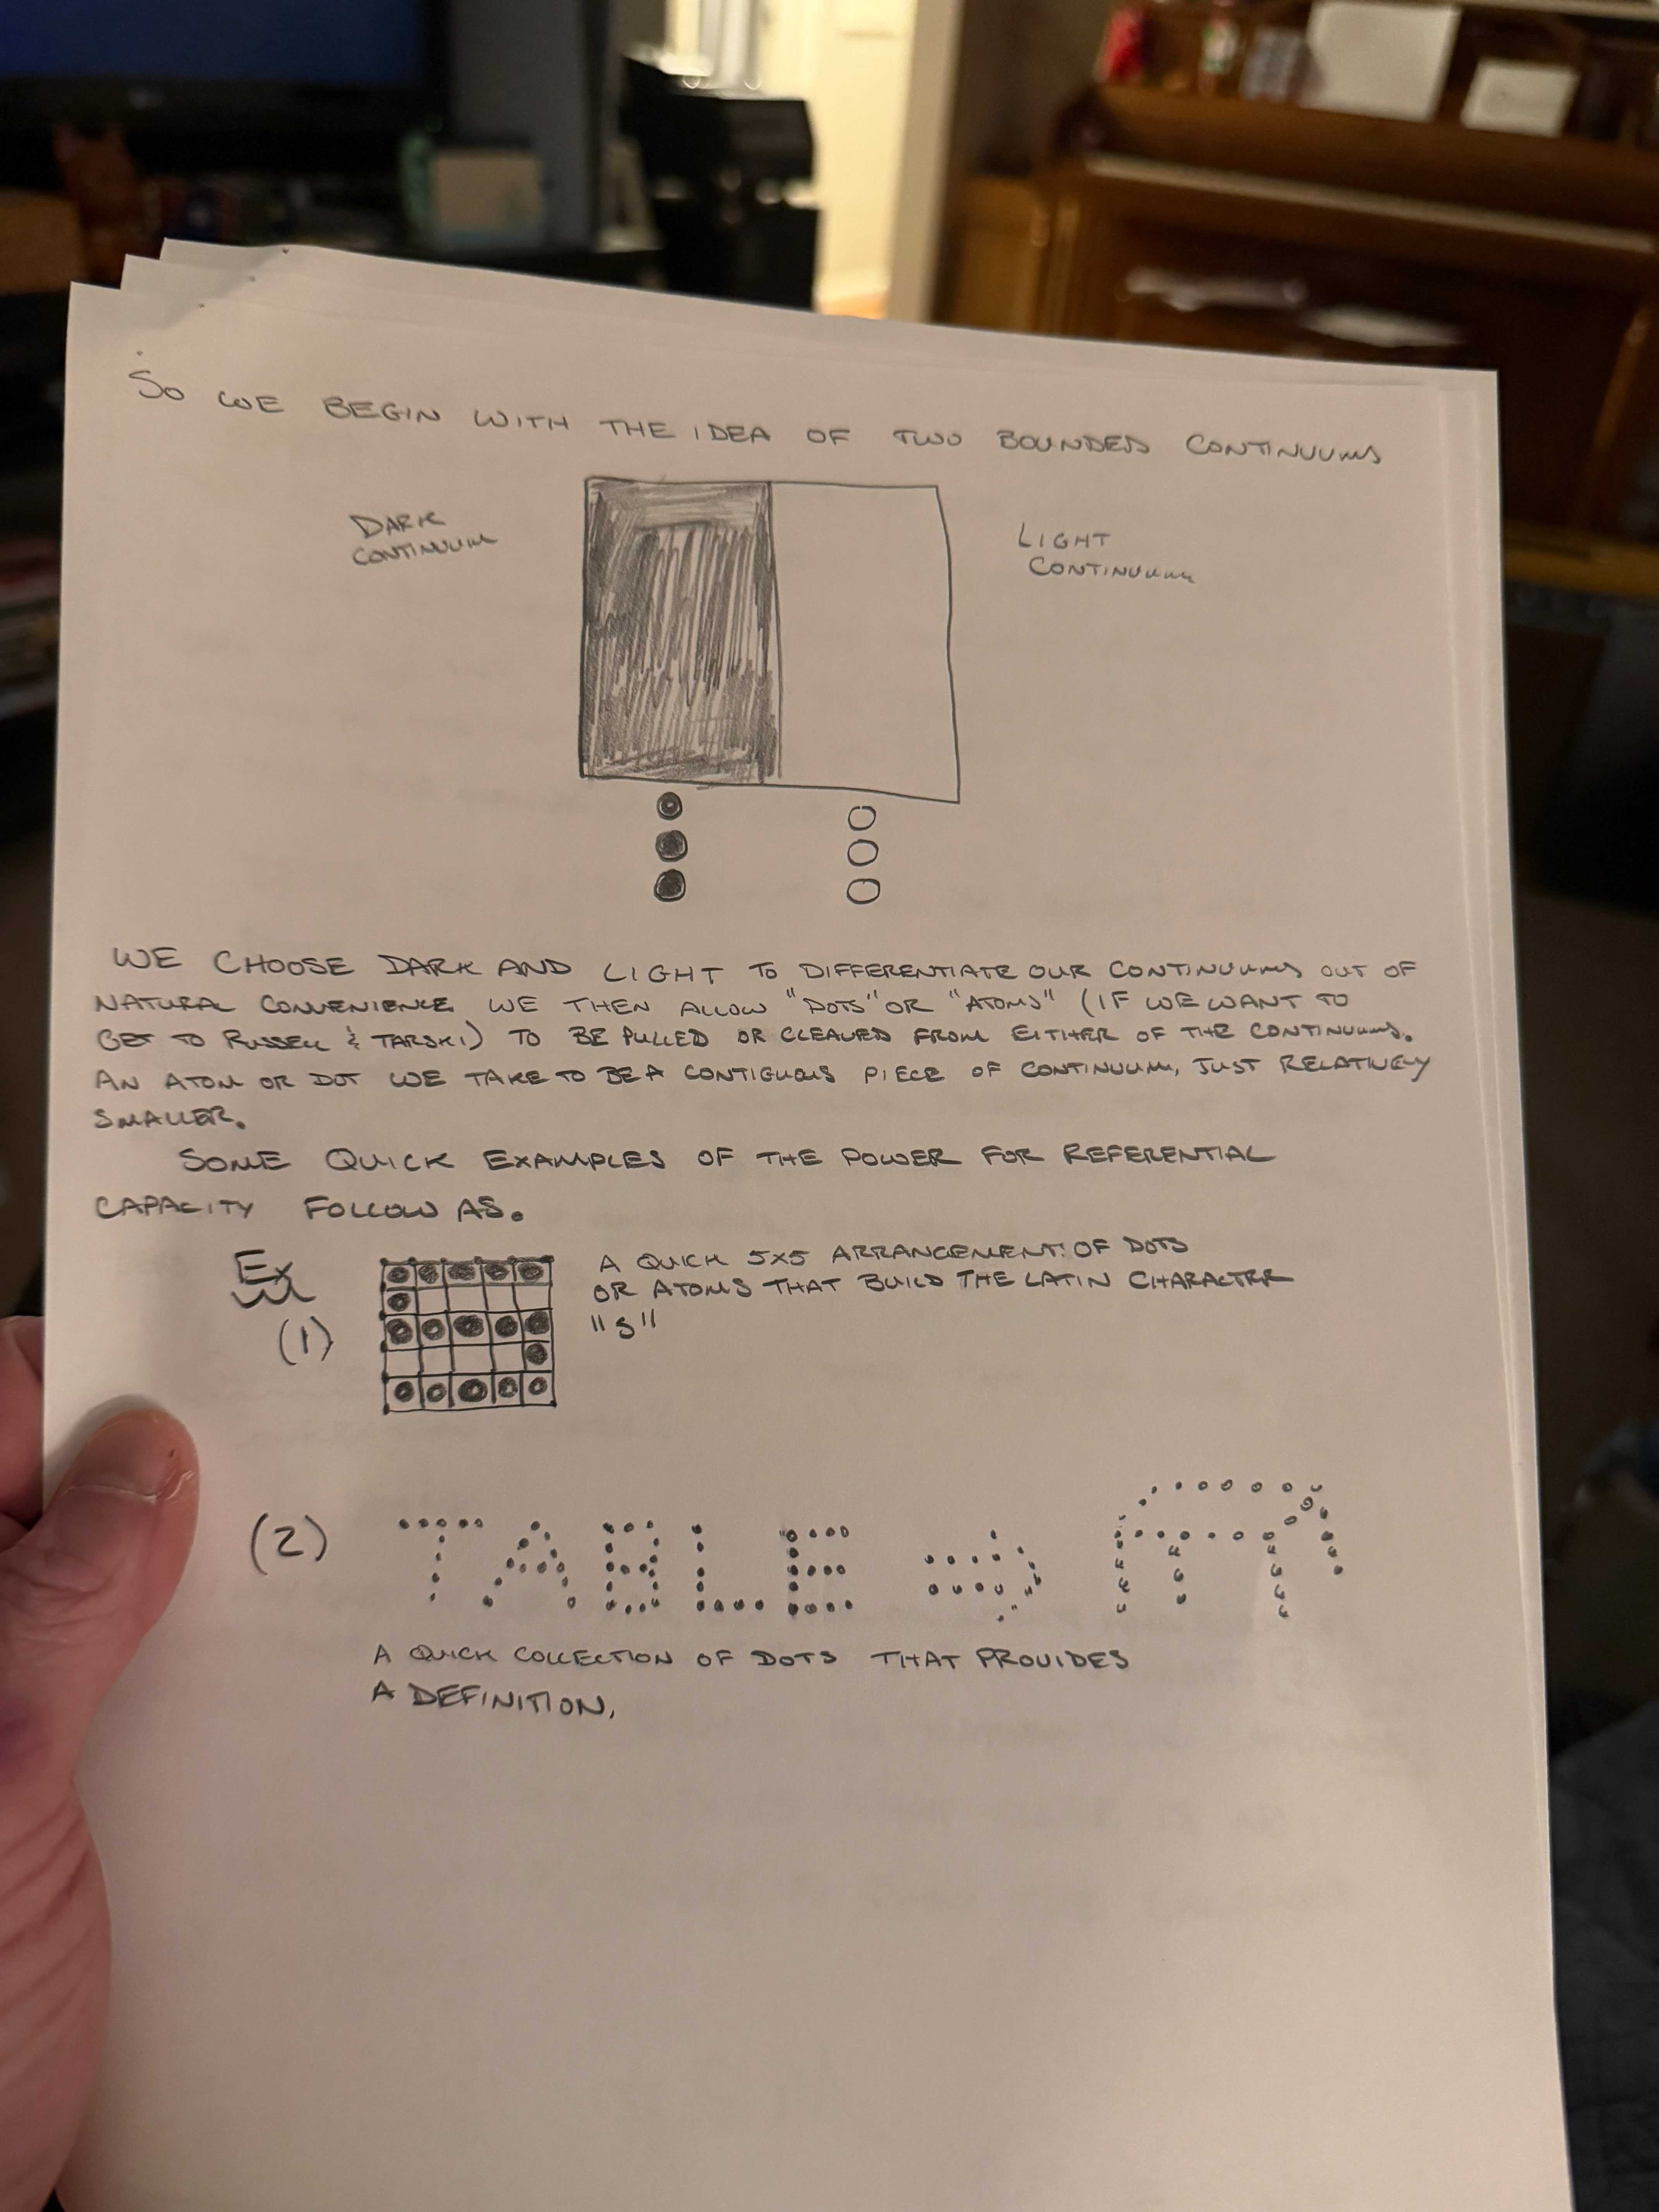
\includegraphics[width=0.4\textwidth]{math2_small.jpeg}
        \caption{Figure 2: A photo of page 2 of this handwritten paper for the purposes of self referentiality}
    \end{figure}

    \newpage

    Once we have the capacity to make characters and references, we can naturally
    build up our logical connectives:

    \[
        \wedge,\ \vee,\ \neg,\ \to,\ \leftrightarrow,\ \equiv,\ \exists,\ \forall,
        \ 0,\ 1,\ S(n)=n+1,\ \{x_0,\ldots,x_n\},\ \{c_0,\ldots,c_n\}.
    \]

    So, this sufficiently builds our language of discourse, call it \(L\), and we
    start by adding \(P:\neg P\) to the language as the first sentence to
    bootstrap the definitions of TRUE, FALSE, AND our logical connectives.

    \textbf{\underline{DEFN}} IF A STATEMENT CAN BE BUILT FROM DOTS OR ATOMS, WE
    CALL IT \underline{WRITABLE}.

    Now WRITABILITY is a fundamental property that both RUSSELL AND TARSKI missed
    in their definitions of the instantiating mechanics of mathematics. IT'S KINDA
    LIKE MISSING ZERO FOR ALL THOSE YEARS.

    \textbf{\underline{QUESTION?}} DO THERE EXIST IDEAS THAT ARE MORE COMPLEX THAN
    WRITABLE?

    \[
        \longrightarrow\quad \text{YES/NO}
    \]

    THEY MAY EXIST IN OUR MINDS, BUT FOR ALL INTENTS AND PURPOSES, IF WE CANNOT
    CONVEY THE IDEA THEN IT'S POINT IS MOOT. SO

    \[
        \boxed{\text{WRITABILITY IS THE BOUND ON MATHEMATICAL LANGUAGE}}
    \]

    THIS EFFECTIVELY IMPLIES THAT THERE IS NO META-LANGUAGE, THERE IS ONLY THE
    LANGUAGE OF DISCOURSE

    \[
        L\subseteq M_L
        \qquad\text{BUT}\qquad
        L\ne M_L.
    \]

    \begin{figure}[htbp]
        \centering
        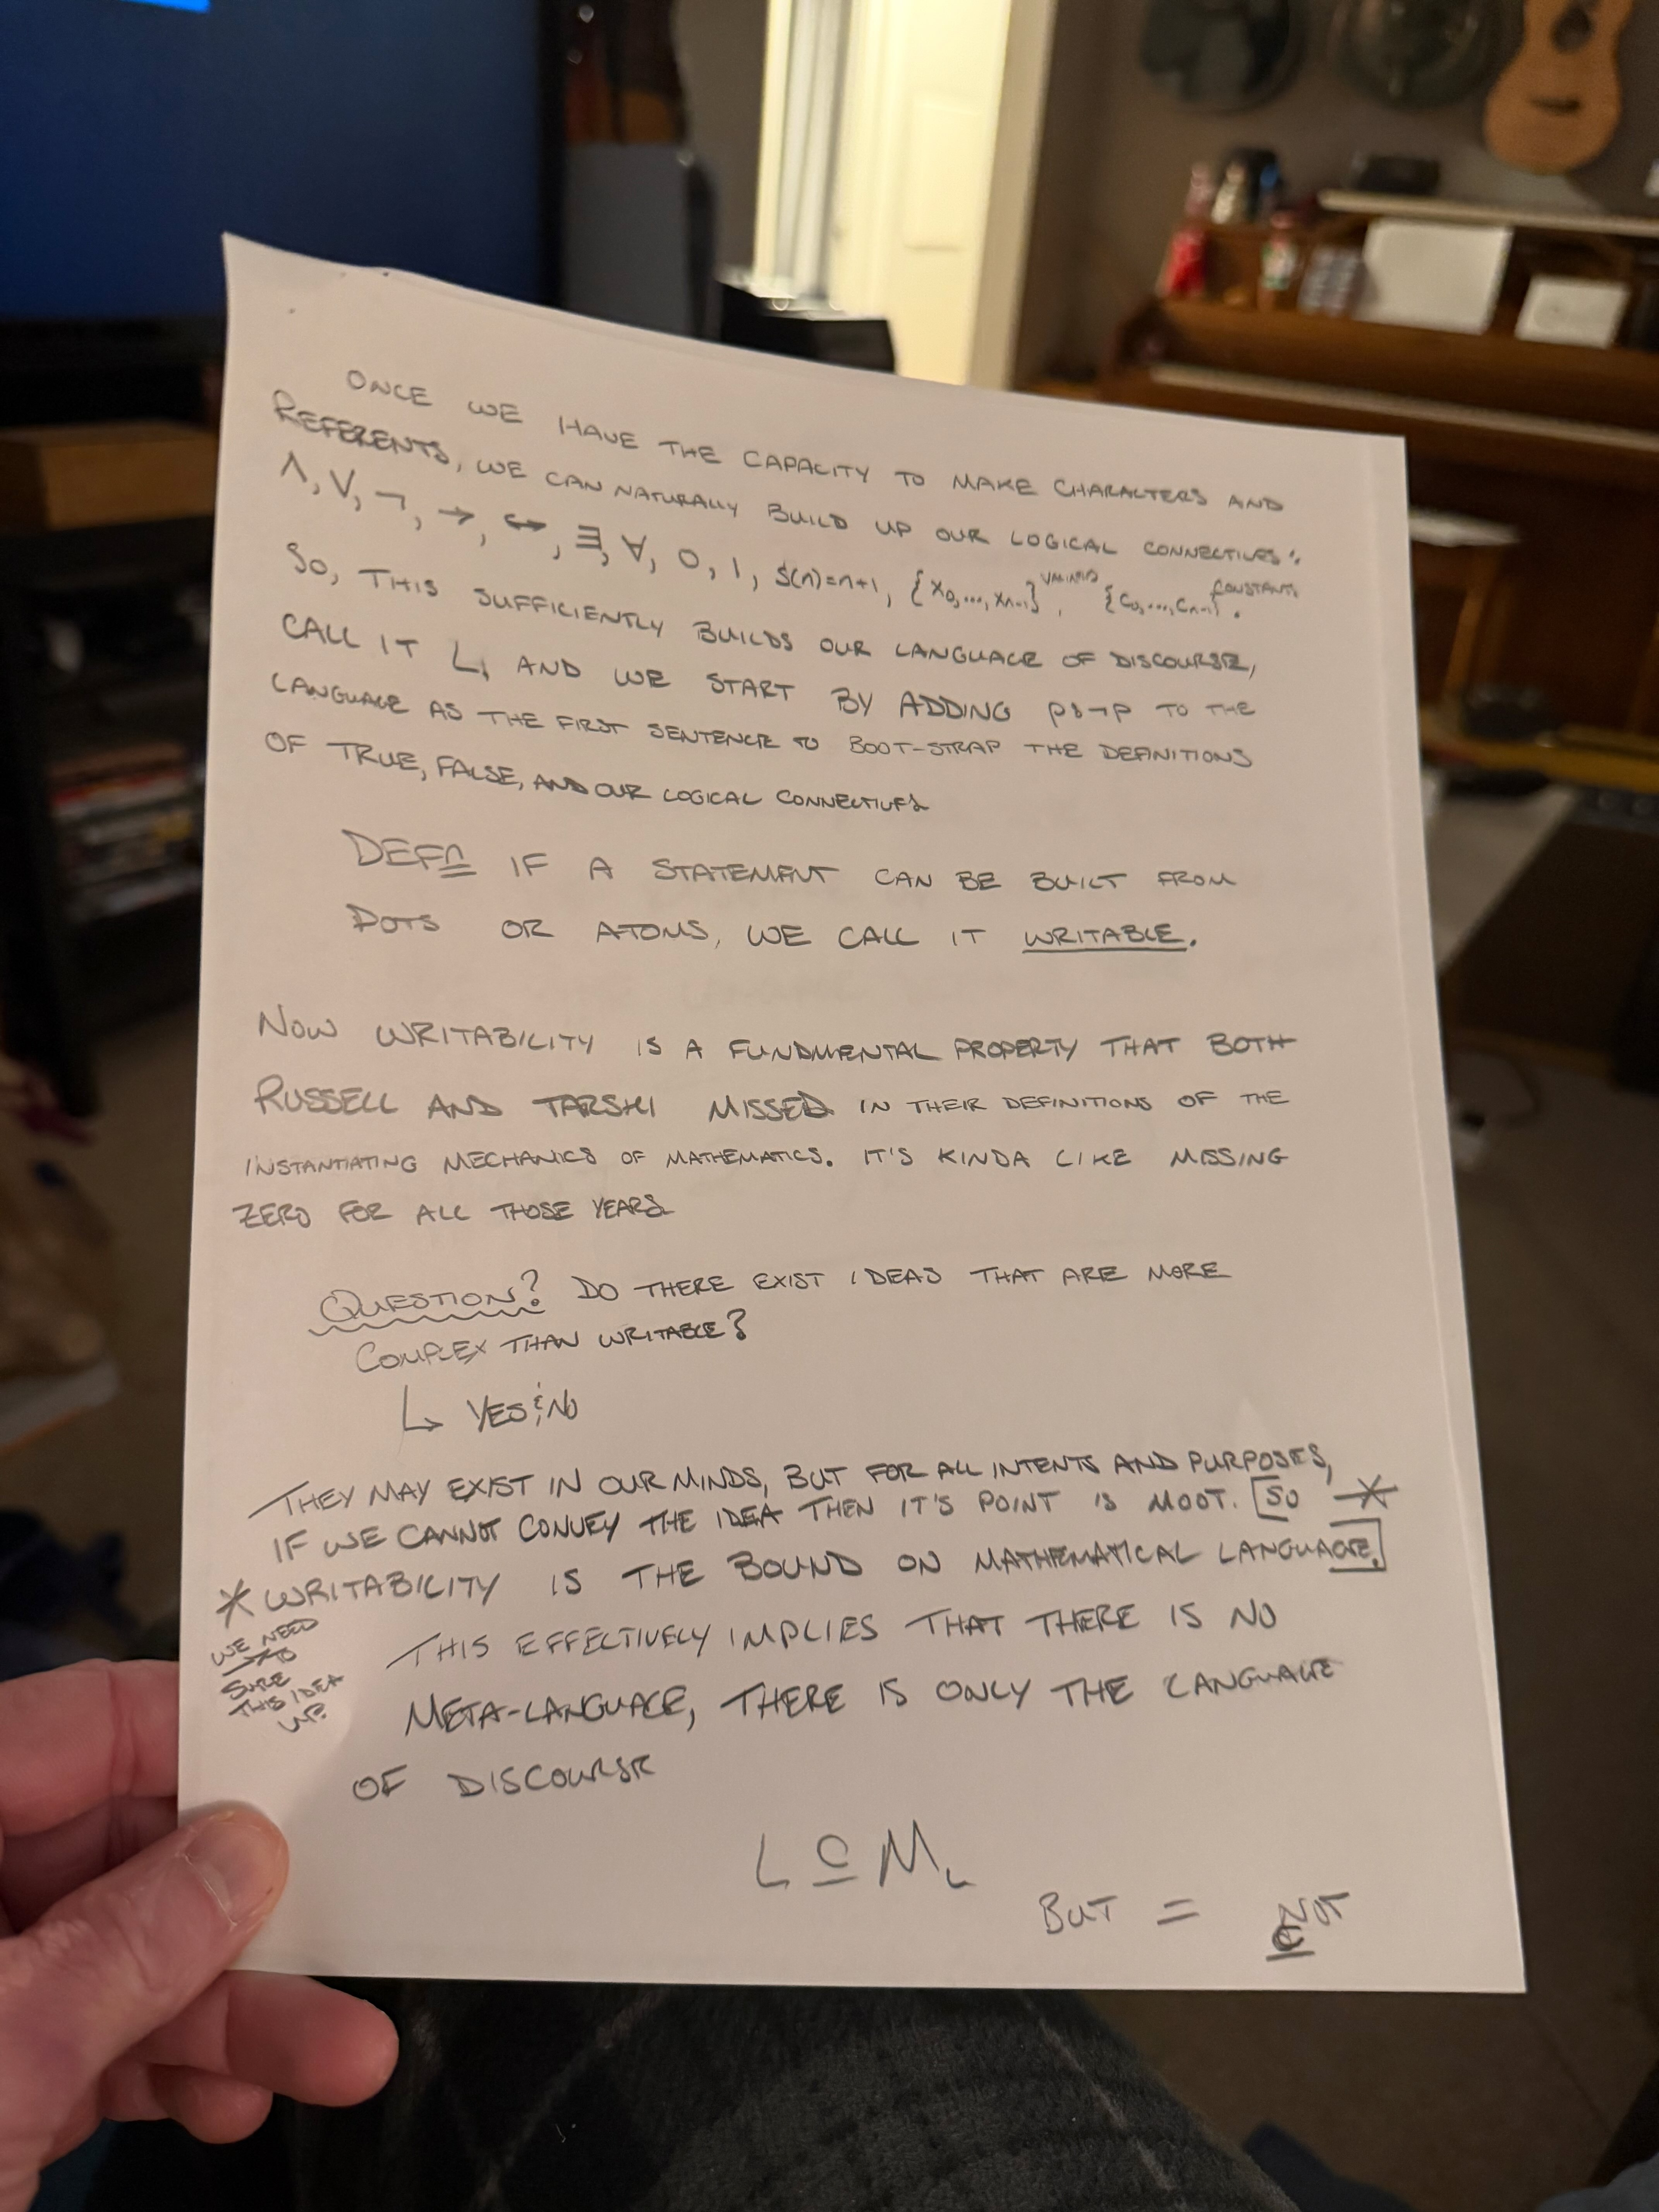
\includegraphics[width=0.4\textwidth]{math3_small.jpeg}
        \caption{Figure 3: A photo of page 3 of this handwritten paper for the purposes of self referentiality}
    \end{figure}

    \newpage

    \[
        \text{BUT NOW}\qquad L=M_L
    \]

    \begin{center}
        SO G\"ODEL'S COMPLETENESS THEOREM\\
        HOLDS
    \end{center}

    \begin{center}
        \begin{tikzpicture}
            \draw[decorate,decoration={brace,amplitude=10pt},thick]
            (0,4.3) -- (0,0);
            \node[anchor=west,align=left,text width=5.6in] at (0.35,2.15) {
                \textbf{CURIOUS!} COMPLETENESS \& INCOMPLETENESS MUST\\[4pt]
                SIMULTANEOUSLY HOLD OVER \(L\) AND \(M_L\)\\[4pt]
                BY THE EXISTENCE OF THE LIAR'S PARADOX,\\[4pt]
                YET THE LANGUAGE DEFINES THE LANGUAGE?
            };
        \end{tikzpicture}
    \end{center}

    \[
        \boxed{\text{HILBERT 2.\quad YES \& NO}}
    \]

    \begin{figure}[htbp]
        \centering
        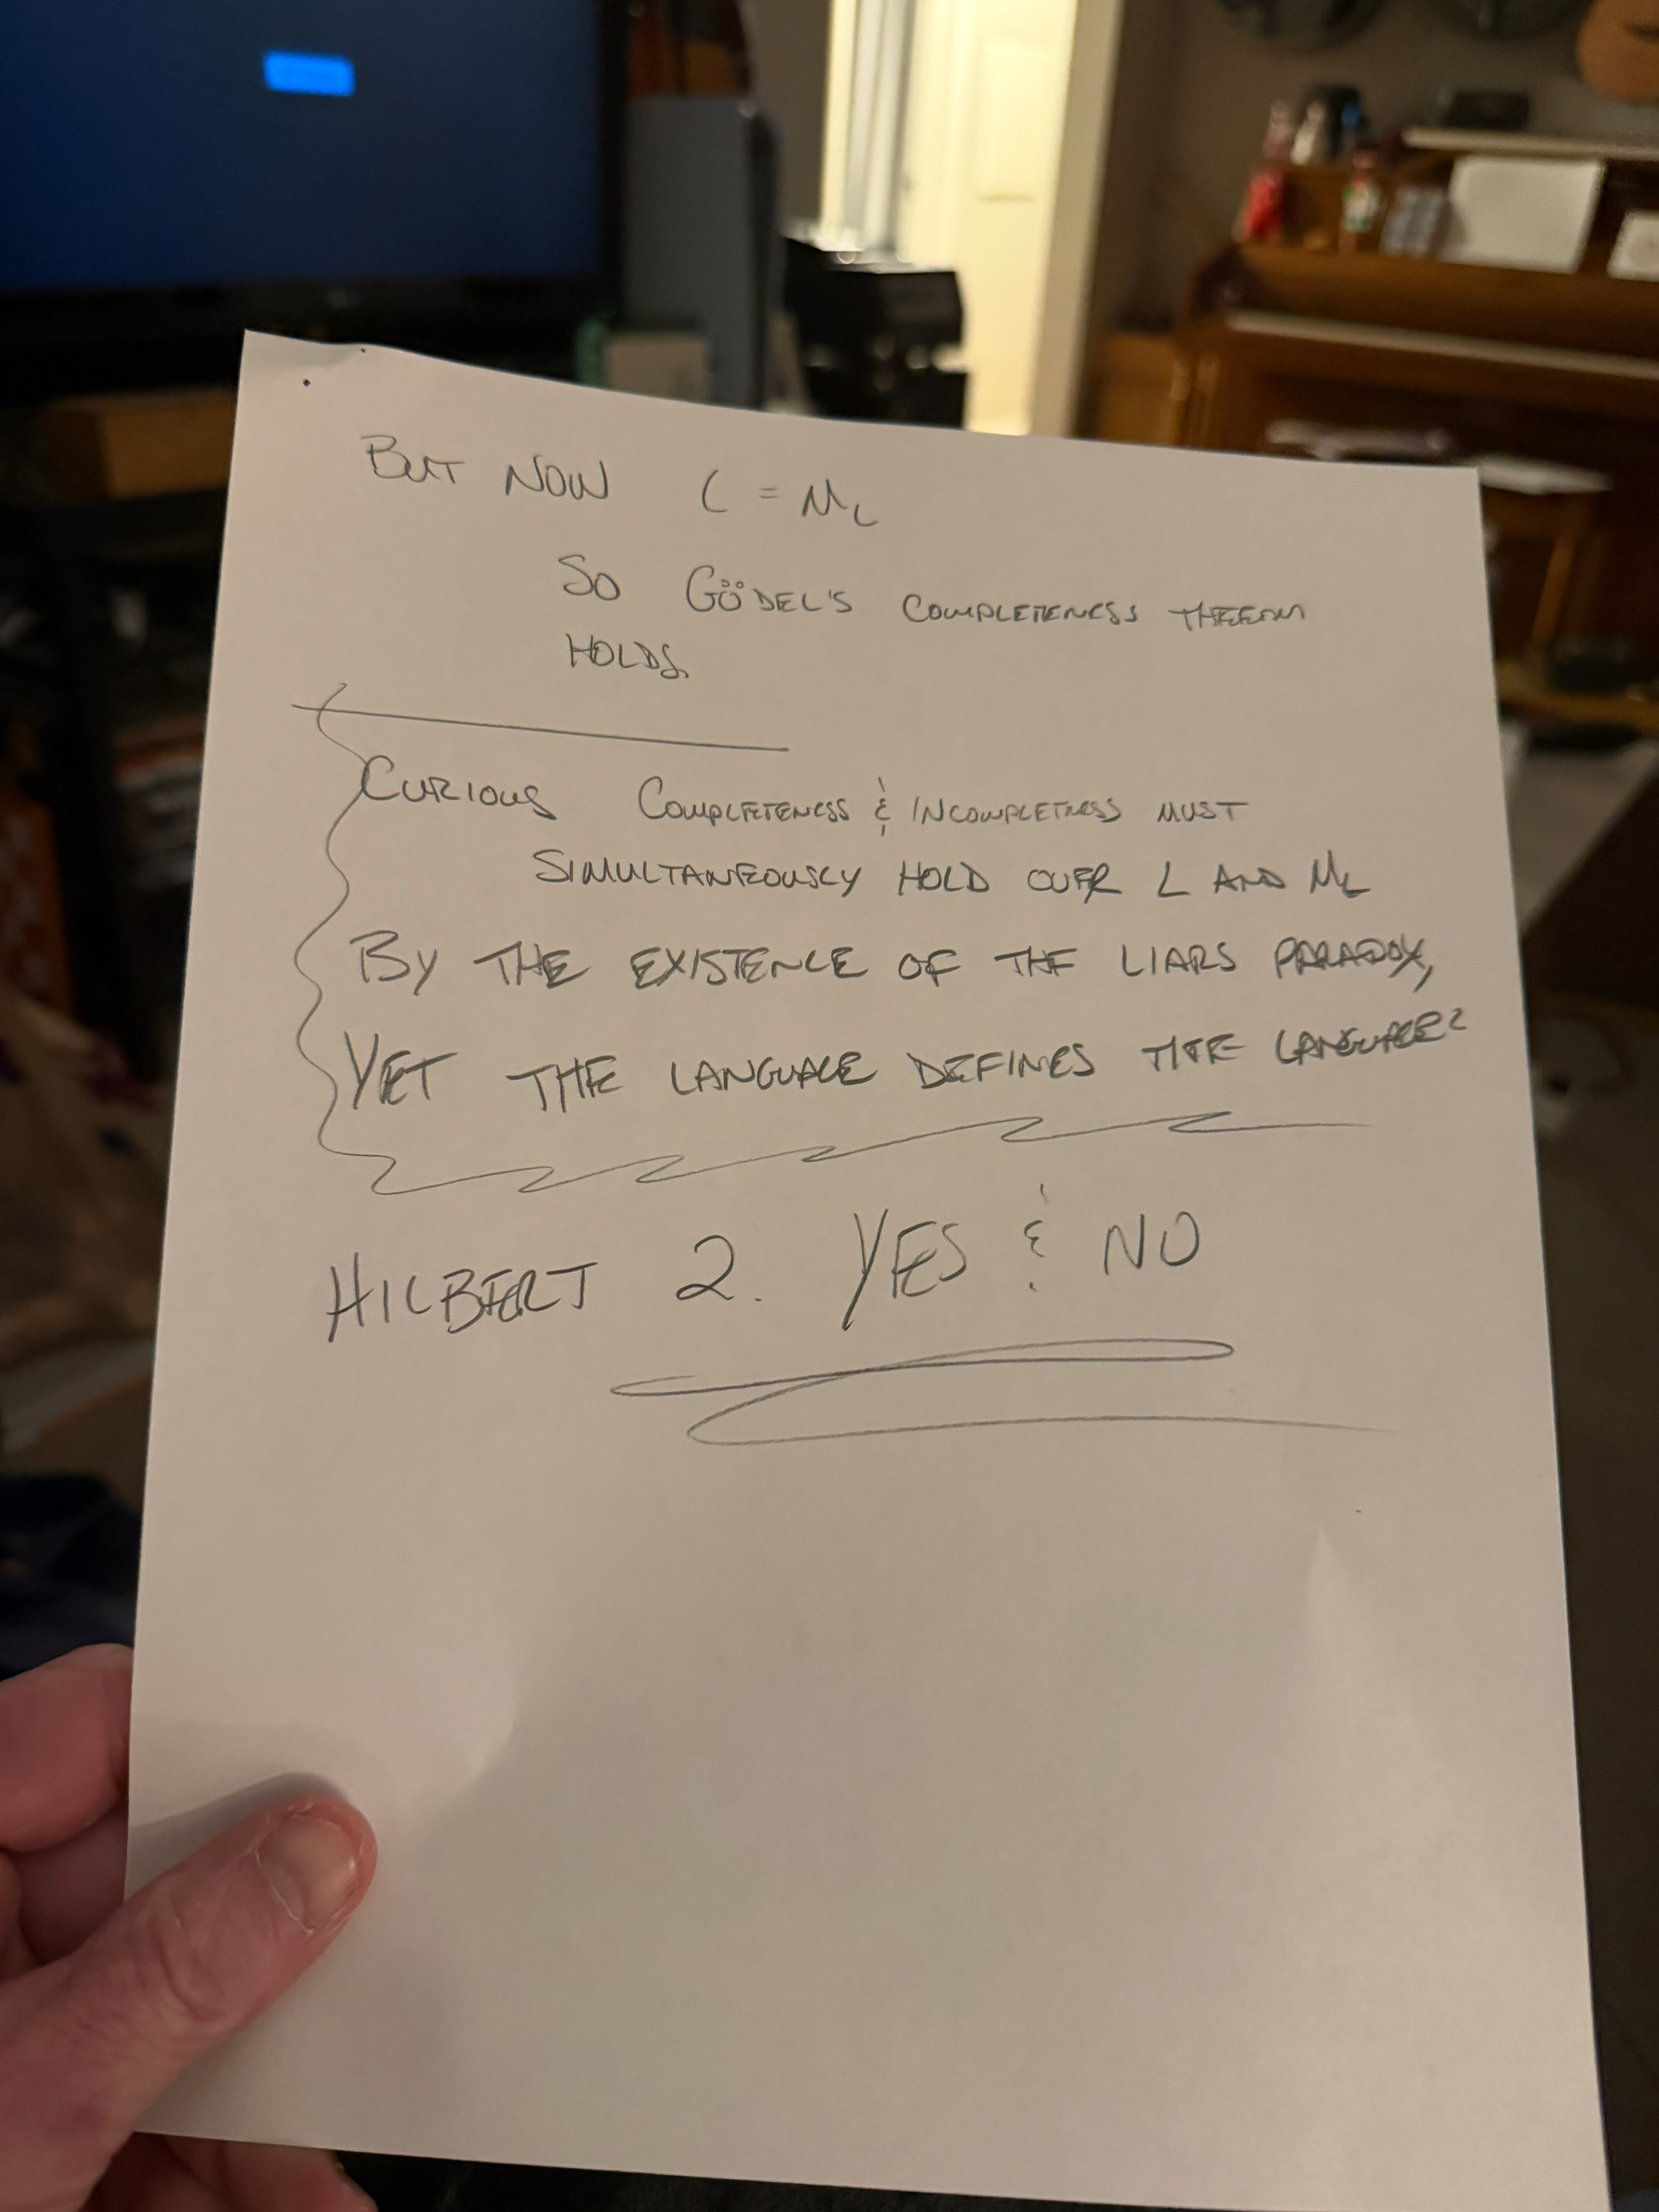
\includegraphics[width=0.4\textwidth]{math4_small.jpeg}
        \caption{Figure 4: A photo of page 4 of this handwritten paper for the purposes of self referentiality}
    \end{figure}

    \clearpage
    \section*{REFERENCES}

    \begin{enumerate}
        \item G. Cantor, ``Ueber eine elementare Frage der
        Mannigfaltigkeitslehre,'' \emph{Jahresbericht der Deutschen
        Mathematiker-Vereinigung} \textbf{1}, 72--78 (1890/91).

        \item P. J. Cohen, ``The independence of the continuum hypothesis,''
        \emph{Proceedings of the National Academy of Sciences} \textbf{50},
        1143--1148 (1963).

        \item P. J. Cohen, \emph{Set Theory and the Continuum Hypothesis}
        (W. A. Benjamin, 1966).

        \item K. G\"odel, \emph{The Consistency of the Axiom of Choice and of the
        Generalized Continuum-Hypothesis with the Axioms of Set Theory}
        (Princeton University Press, 1940).

        \item K. G\"odel, ``\"Uber formal unentscheidbare S\"atze der
        \emph{Principia Mathematica} und verwandter Systeme I,''
        \emph{Monatshefte f\"ur Mathematik und Physik} \textbf{38}, 173--198
        (1931).

        \item K. G\"odel, ``Die Vollst\"andigkeit der Axiome des logischen
        Funktionenkalk\"uls,'' \emph{Monatshefte f\"ur Mathematik und Physik}
        \textbf{37}, 349--360 (1930).

        \item D. Hilbert, ``Mathematische Probleme,'' \emph{Nachrichten von der
        K\"oniglichen Gesellschaft der Wissenschaften zu G\"ottingen,
            Mathematisch-Physikalische Klasse}, 253--297 (1900).

        \item A. Tarski, ``Der Wahrheitsbegriff in den formalisierten Sprachen,''
        \emph{Studia Philosophica} \textbf{1}, 261--405 (1936).

        \item A. M. Turing, ``On computable numbers, with an application to the
        Entscheidungsproblem,'' \emph{Proceedings of the London Mathematical
        Society} s2-\textbf{42}, 230--265 (1937).

        \item A. N. Whitehead and B. Russell, \emph{Principia Mathematica},
        vols. 1--3 (Cambridge University Press, 1910--1913).
    \end{enumerate}

\end{document}
% End of science_template.tex